%\documentclass[crop,tikz,convert={outext=.svg,command=\unexpanded{pdf2svg \infile\space\ou
%tfile}},multi=false]{standalone}[2012/04/13]

\documentclass[crop,tikz]{standalone}[2012/04/13]

\usepackage{pgf}

\usetikzlibrary{arrows,automata}
\usepackage[latin1]{inputenc}
\begin{document}
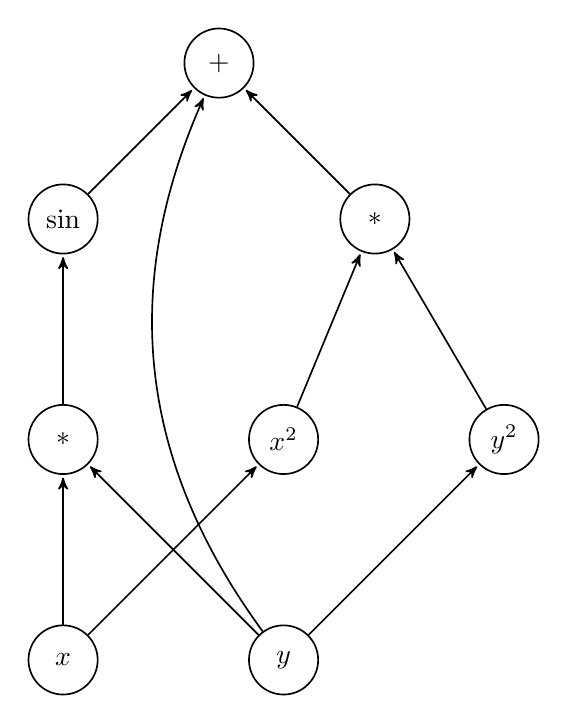
\begin{tikzpicture}[->,>=stealth',shorten >=1pt,auto,node distance=2.8cm,
                    semithick]
 % \tikzstyle{every state}=[fill=red,draw=none,text=white]

  \node[state]         (A)                    {$+$};
  \node[state]         (B) [below left of=A] {$\sin$};
  \node[state]         (C) [below right of=A] {$*$};
  \node[state]         (D) [below of=B]       {$*$};
  \node[state]         (E) [right of=D] {$x^2$};
  \node[state]         (F) [right of=E]       {$y^2$};
  \node[state]         (G) [below of=D]       {$x$};
  \node[state]         (H) [right of=G]       {$y$};
  

  
  \path (B) edge              node {} (A);
  \path (C) edge              node {} (A);
  \path (E) edge              node {} (C);
  \path (F) edge              node {} (C);
  \path (D) edge              node {} (B);
  \path (G) edge              node {} (D);
  \path (G) edge              node {} (E);
  \path (H) edge              node {} (D);
  \path (H) edge              node {} (F);
  \path (H) edge [bend left]  node {} (A);

  %           edge              node {1,1,R} (C)
  %       (B) edge [loop above] node {1,1,L} (B)
  %           edge              node {0,1,L} (C)
  %       (C) edge              node {0,1,L} (D)
  %           edge [bend left]  node {1,0,R} (E)
  %       (D) edge [loop below] node {1,1,R} (D)
  %           edge              node {0,1,R} (A)
  %       (E) edge [bend left]  node {1,0,R} (A);
\end{tikzpicture}

\end{document}